\documentclass[a4paper]{jsarticle}
\usepackage{graphicx}
\usepackage{amsmath,amssymb,bm}
\usepackage{algorithm,algpseudocode}

\flushbottom
\sloppy

%%% paper size = A4
\setlength{\paperwidth}{210mm}
\setlength{\paperheight}{297mm}

%%% truncate offset
\setlength{\voffset}{0mm}
\setlength{\hoffset}{0mm}

%%% text bounding size
\setlength{\textwidth}{\paperwidth}
\addtolength{\textwidth}{-30mm}
\setlength{\textheight}{\paperheight}
\addtolength{\textheight}{-60mm}

%%% text margin
\setlength{\topmargin}{-1in}
\addtolength{\topmargin}{20mm}
\setlength{\headheight}{0mm}
\setlength{\headsep}{0mm}
\setlength{\footskip}{10mm}

%\setlength{\oddsidemargin}{-30pt}
\setlength{\oddsidemargin}{-1in}
\addtolength{\oddsidemargin}{15mm}
\setlength{\columnsep}{7mm}

\title{\bf 最小包含球(Bounding Ball, Smallest Enclosing Ball)を求めるエレガントなアルゴリズム}
\author{\Large{\bf 杉原 知道}}
\date{}

\begin{document}
\maketitle
\vspace{-\baselineskip}

\section{はじめに}

$n$個の点から成る点群$\mathcal{P}=\{\boldsymbol{p}_{i}|i=1\sim N\}$を内部および表面上に全て含む球のうち,
最小半径のものを{\bf 最小包含球}と呼びます.
最も単純な包含立体の一つであり,
領域判定や干渉判定などのいろいろな場面で有用なものです.
これを求めるアルゴリズムは幾つかありますが,
本記事ではその中でもエレガントな,
次の論文で提案されているものを解説します.

Emo Welzl, Smallest enclosing disks (balls and ellipsoids), in New Results and New Trends in Computer Science, Lecture Notes in Computer Science, Springer-Verlag, pp. 359--370, 1991.

以下では,
点群$\mathcal{P}$に対する最小包含球を$\mathcal{BB}(\mathcal{P})$と表すことにします.


\section{点の数$N\leq 4$のときの最小包含球}

点の数$N=1$のときは,
$\mathcal{BB}(\mathcal{P})$は$\mathcal{P}$に含まれるただ一つの点を中心とする半径$0$の球となります.
最小包含球が実用上の意味を持つのは$N\geq 2$の場合で,このとき次の命題$\star$が成り立ちます.

\begin{quote}
命題$\star$)
$N\geq 2$のとき,
$\mathcal{BB}(\mathcal{P})$は次の3つの条件のうちいずれかを必ず満たす.
\begin{enumerate}
\item{$\mathcal{P}$に含まれるある2点を直径の両端に持つ.}
\item{$\mathcal{P}$に含まれるある3点から成る三角形の外接円を最大断面とする.}
\item{$\mathcal{P}$に含まれるある4点から成る四面体の外接球である.}
\end{enumerate}
\end{quote}

1つめの条件を満たす球は${}_{N}C_{2}$個,
2つめの条件を満たす球は${}_{N}C_{3}$個,
3つめの条件を満たす球は${}_{N}C_{4}$個あります.
$N\leq 4$のときは高々${}_{4}C_{2}+{}_{4}C_{3}+{}_{4}C_{4}=10$通りの候補を実際に求め,
その中から最小半径のものを選べば良いわけです.

具体的にそれぞれの球を求めてみます.
データ構造としては,球は中心座標$\boldsymbol{p}_{\mathrm{C}}$と半径$r$の組で表されます.

\subsection{$\boldsymbol{p}_{i}$と$\boldsymbol{p}_{j}$を直径の両端点とする球}

これは単純に,中心座標$\boldsymbol{p}_{\mathrm{C}}=\frac{\displaystyle\boldsymbol{p}_{i}+\boldsymbol{p}_{j}}{\displaystyle 2}$,半径$r=\frac{\displaystyle \|\boldsymbol{p}_{i}-\boldsymbol{p}_{j}\|}{\displaystyle 2}$と求まります.

\subsection{$\boldsymbol{p}_{i}$,$\boldsymbol{p}_{j}$,$\boldsymbol{p}_{k}$を頂点とする三角形の外接円を最大断面とする球}

\begin{figure*}[h]
\centering
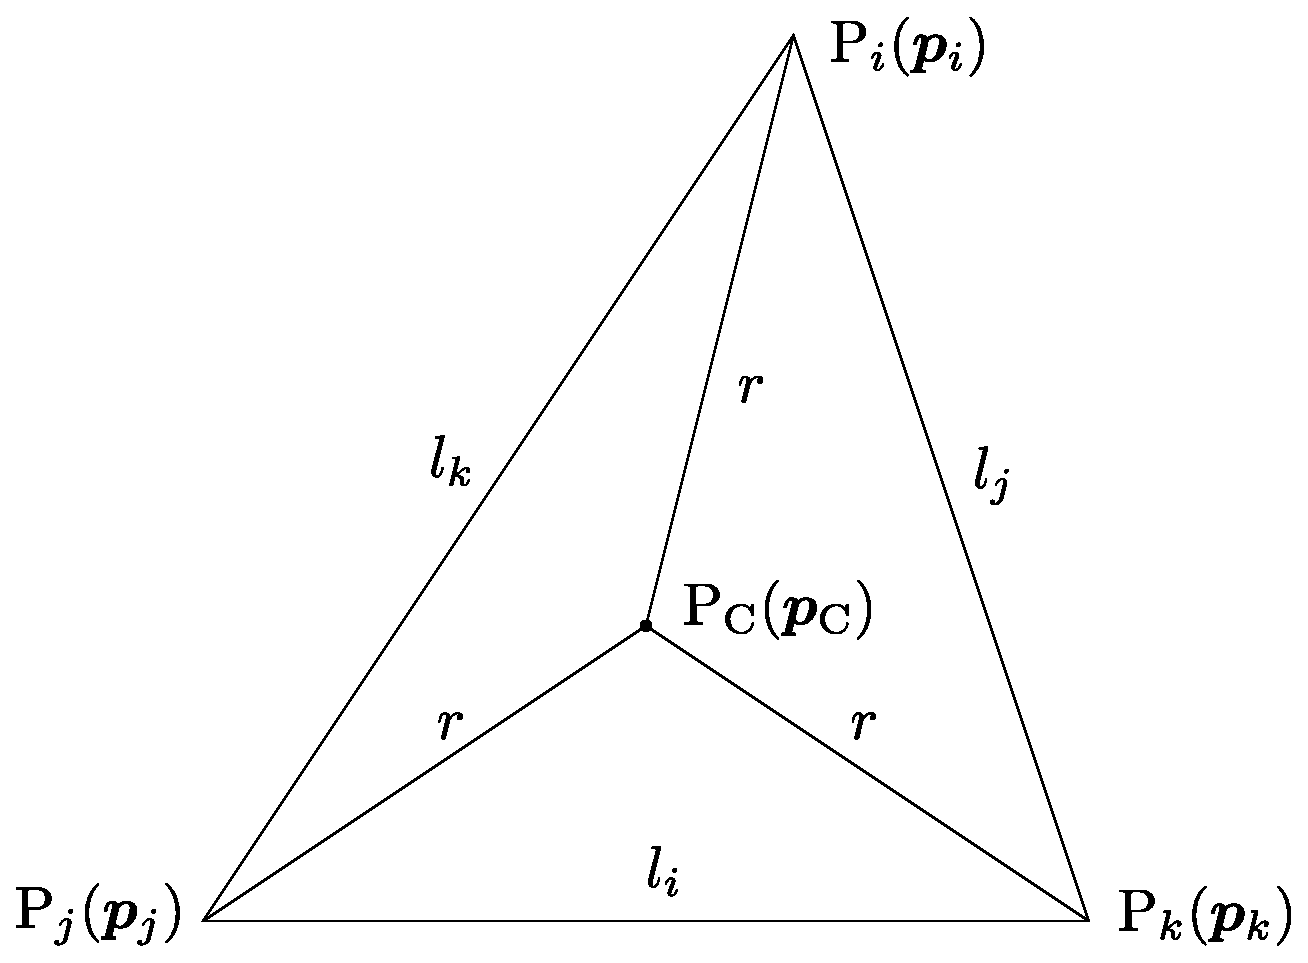
\includegraphics[width=.6\textwidth]{fig/circumcenter_triangle.eps}
\end{figure*}

上図のように,三角形の頂点を$\mathrm{P}_{i}(\boldsymbol{p}_{i})$,$\mathrm{P}_{j}(\boldsymbol{p}_{j})$,$\mathrm{P}_{k}(\boldsymbol{p}_{k})$,
中心を$\mathrm{P}_{\mathrm{C}}(\boldsymbol{p}_{\mathrm{C}})$とそれぞれおきます.
$s_{i}=\triangle\mathrm{P}_{\mathrm{C}}\mathrm{P}_{j}\mathrm{P}_{k}$,
$s_{j}=\triangle\mathrm{P}_{\mathrm{C}}\mathrm{P}_{k}\mathrm{P}_{i}$,
$s_{k}=\triangle\mathrm{P}_{\mathrm{C}}\mathrm{P}_{i}\mathrm{P}_{j}$とそれぞれおいたとき,
\begin{align*}
\boldsymbol{p}_{\mathrm{C}}=\frac{s_{i}\boldsymbol{p}_{i}+s_{j}\boldsymbol{p}_{j}+s_{k}\boldsymbol{p}_{k}}{s_{i}+s_{j}+s_{k}}
\end{align*}
であることが知られています.
円周角の定理より
$\angle\mathrm{P}_{j}\mathrm{P}_{\mathrm{C}}\mathrm{P}_{k}=2\angle\mathrm{P}_{j}\mathrm{P}_{i}\mathrm{P}_{k}$,
$\angle\mathrm{P}_{k}\mathrm{P}_{\mathrm{C}}\mathrm{P}_{i}=2\angle\mathrm{P}_{k}\mathrm{P}_{j}\mathrm{P}_{i}$,
$\angle\mathrm{P}_{i}\mathrm{P}_{\mathrm{C}}\mathrm{P}_{j}=2\angle\mathrm{P}_{i}\mathrm{P}_{k}\mathrm{P}_{j}$ですので,
\begin{align*}
s_{i}=\frac{1}{2}r^{2}\sin 2\angle\mathrm{P}_{j}\mathrm{P}_{i}\mathrm{P}_{k}
\\
s_{j}=\frac{1}{2}r^{2}\sin 2\angle\mathrm{P}_{k}\mathrm{P}_{j}\mathrm{P}_{i}
\\
s_{k}=\frac{1}{2}r^{2}\sin 2\angle\mathrm{P}_{i}\mathrm{P}_{k}\mathrm{P}_{j}
\end{align*}
さらに
$l_{i}=\|\boldsymbol{p}_{j}-\boldsymbol{p}_{k}\|$,
$l_{j}=\|\boldsymbol{p}_{k}-\boldsymbol{p}_{i}\|$,
$l_{k}=\|\boldsymbol{p}_{i}-\boldsymbol{p}_{j}\|$とおくと,
正弦定理
\begin{align*}
\sin\angle\mathrm{P}_{j}\mathrm{P}_{i}\mathrm{P}_{k}=l_{i}/2r
\\
\sin\angle\mathrm{P}_{k}\mathrm{P}_{j}\mathrm{P}_{i}=l_{j}/2r
\\
\sin\angle\mathrm{P}_{i}\mathrm{P}_{k}\mathrm{P}_{j}=l_{k}/2r
\end{align*}
および余弦定理
\begin{align*}
\cos\angle\mathrm{P}_{j}\mathrm{P}_{i}\mathrm{P}_{k}=\frac{l_{j}^{2}+l_{k}^{2}-l_{i}^{2}}{2l_{j}l_{k}}
\\
\cos\angle\mathrm{P}_{k}\mathrm{P}_{j}\mathrm{P}_{i}=\frac{l_{k}^{2}+l_{i}^{2}-l_{j}^{2}}{2l_{k}l_{i}}
\\
\cos\angle\mathrm{P}_{i}\mathrm{P}_{k}\mathrm{P}_{j}=\frac{l_{i}^{2}+l_{j}^{2}-l_{k}^{2}}{2l_{i}l_{j}}
\end{align*}
より,倍角公式を使えば
\begin{align*}
s_{i}=\frac{1}{2}r^{2}\cdot\frac{l_{i}}{2r}\cdot\frac{l_{j}^{2}+l_{k}^{2}-l_{i}^{2}}{2l_{j}l_{k}}
\\
s_{j}=\frac{1}{2}r^{2}\cdot\frac{l_{j}}{2r}\cdot\frac{l_{k}^{2}+l_{i}^{2}-l_{j}^{2}}{2l_{k}l_{i}}
\\
s_{k}=\frac{1}{2}r^{2}\cdot\frac{l_{k}}{2r}\cdot\frac{l_{i}^{2}+l_{j}^{2}-l_{k}^{2}}{2l_{i}l_{j}}
\end{align*}
となります.
中心座標を求める際には,これらの比だけが意味を持つので,
\begin{align*}
s_{i}=l_{i}^{2}(l_{j}^{2}+l_{k}^{2}-l_{i}^{2})
\\
s_{j}=l_{j}^{2}(l_{k}^{2}+l_{i}^{2}-l_{j}^{2})
\\
s_{k}=l_{k}^{2}(l_{i}^{2}+l_{j}^{2}-l_{k}^{2})
\end{align*}
としても問題ありません.
これらを上の式に代入すれば,$\boldsymbol{p}_{\mathrm{C}}$を得ます.
半径は,$r=\|\boldsymbol{p}_{i}-\boldsymbol{p}_{\mathrm{C}}\|$と求まります.

\subsection{$\boldsymbol{p}_{i}$,$\boldsymbol{p}_{j}$,$\boldsymbol{p}_{k}$,$\boldsymbol{p}_{l}$を頂点とする四面体の外接球}

頂点を$\mathrm{P}_{i}(\boldsymbol{p}_{i})$,$\mathrm{P}_{j}(\boldsymbol{p}_{j})$,$\mathrm{P}_{k}(\boldsymbol{p}_{k})$,$\mathrm{P}_{l}(\boldsymbol{p}_{l})$,
中心を$\mathrm{P}_{\mathrm{C}}(\boldsymbol{p}_{\mathrm{C}})$とそれぞれおきます.
外接球の中心は,
辺$\overline{\mathrm{P}_{i}\mathrm{P}_{l}}$の二等分面,
辺$\overline{\mathrm{P}_{j}\mathrm{P}_{l}}$の二等分面,
辺$\overline{\mathrm{P}_{k}\mathrm{P}_{l}}$の二等分面の交点として求まります.
このことから,
$\boldsymbol{e}_{i}=\boldsymbol{p}_{i}-\boldsymbol{p}_{l}$,
$\boldsymbol{e}_{j}=\boldsymbol{p}_{j}-\boldsymbol{p}_{l}$,
$\boldsymbol{e}_{k}=\boldsymbol{p}_{k}-\boldsymbol{p}_{l}$,
$\boldsymbol{e}_{\mathrm{C}}=\boldsymbol{p}_{\mathrm{C}}-\boldsymbol{p}_{l}$とそれぞれおくと,次が成り立ちます.
\begin{align*}
\boldsymbol{e}_{i}^{\mathrm{T}}\boldsymbol{e}_{\mathrm{C}}=\frac{1}{2}\|\boldsymbol{e}_{i}\|^{2}
\\
\boldsymbol{e}_{j}^{\mathrm{T}}\boldsymbol{e}_{\mathrm{C}}=\frac{1}{2}\|\boldsymbol{e}_{j}\|^{2}
\\
\boldsymbol{e}_{k}^{\mathrm{T}}\boldsymbol{e}_{\mathrm{C}}=\frac{1}{2}\|\boldsymbol{e}_{k}\|^{2}
\end{align*}
これらは,次のようにまとめられます.
\begin{align*}
\begin{bmatrix} \boldsymbol{e}_{i}^{\mathrm{T}} \\ \boldsymbol{e}_{j}^{\mathrm{T}} \\ \boldsymbol{e}_{k}^{\mathrm{T}} \end{bmatrix}
\boldsymbol{e}_{\mathrm{C}}=
\frac{1}{2}
\begin{bmatrix} \|\boldsymbol{e}_{i}\|^{2} \\ \|\boldsymbol{e}_{j}\|^{2} \\ \|\boldsymbol{e}_{k}\|^{2} \end{bmatrix}
\end{align*}
これは$\boldsymbol{e}_{\mathrm{C}}$について次のように直接的に解けます.
\begin{align*}
\boldsymbol{e}_{\mathrm{C}}=
\frac{1}{2}
\begin{bmatrix} \boldsymbol{e}_{i}^{\mathrm{T}} \\ \boldsymbol{e}_{j}^{\mathrm{T}} \\ \boldsymbol{e}_{k}^{\mathrm{T}} \end{bmatrix}^{-1}
\begin{bmatrix} \|\boldsymbol{e}_{i}\|^{2} \\ \|\boldsymbol{e}_{j}\|^{2} \\ \|\boldsymbol{e}_{k}\|^{2} \end{bmatrix}
=
\frac{1}{2\left[\boldsymbol{e}_{i}~\boldsymbol{e}_{j}~\boldsymbol{e}_{k}\right]}
\begin{bmatrix}
\boldsymbol{e}_{j}\times\boldsymbol{e}_{k} & \boldsymbol{e}_{k}\times\boldsymbol{e}_{i} & \boldsymbol{e}_{i}\times\boldsymbol{e}_{j}
\end{bmatrix}
\begin{bmatrix} \|\boldsymbol{e}_{i}\|^{2} \\ \|\boldsymbol{e}_{j}\|^{2} \\ \|\boldsymbol{e}_{k}\|^{2} \end{bmatrix}
\\
=
\frac{
\|\boldsymbol{e}_{i}\|^{2}\boldsymbol{e}_{j}\times\boldsymbol{e}_{k}
+\|\boldsymbol{e}_{j}\|^{2}\boldsymbol{e}_{k}\times\boldsymbol{e}_{i}
+\|\boldsymbol{e}_{k}\|^{2}\boldsymbol{e}_{i}\times\boldsymbol{e}_{j}
}
{2\left[\boldsymbol{e}_{i}~\boldsymbol{e}_{j}~\boldsymbol{e}_{k}\right]}
\end{align*}
ただし,
$\left[\boldsymbol{e}_{i}~\boldsymbol{e}_{j}~\boldsymbol{e}_{k}\right]
=\boldsymbol{e}_{i}^{\mathrm{T}}(\boldsymbol{e}_{j}\times\boldsymbol{e}_{k})
=\boldsymbol{e}_{j}^{\mathrm{T}}(\boldsymbol{e}_{k}\times\boldsymbol{e}_{i})
=\boldsymbol{e}_{k}^{\mathrm{T}}(\boldsymbol{e}_{i}\times\boldsymbol{e}_{j})$
はスカラー三重積と呼ばれます.
中心座標は$\boldsymbol{p}_{\mathrm{C}}=\boldsymbol{p}_{l}+\boldsymbol{e}_{\mathrm{C}}$となります.
半径は,前のケースと同様に
\begin{align*}
r=\|\boldsymbol{p}_{i}-\boldsymbol{p}_{\mathrm{C}}\|
\end{align*}
と求まります.

\section{$N\geq 5$のときの最小包含球}

$N\geq 5$のときは,
次のような再帰的手続きを定義します.
ただし,$\mathcal{P}_{n}=\{\boldsymbol{p}_{i}|i=1\sim n\}$とおいています($\mathcal{P}_{n}=\mathcal{P}_{n-1}\cup\left\{\boldsymbol{p}_{n}\right\}$,$\mathcal{P}=\mathcal{P}_{N}$です).
\begin{algorithm}[h]
\caption{\textsc{BoundingBall}$(\mathcal{P}_{n})\rightarrow\mathcal{BB}(\mathcal{P}_{n})$}
\begin{algorithmic}[1]
\If{$n\leq 4$}
  \State {\bf Return} \textsc{BoundingBallDirect}$(\mathcal{P}_{n})$
\EndIf
\State $\mathcal{BB}(\mathcal{P}_{n-1})\leftarrow$\textsc{BoundingBall}$(\mathcal{P}_{n-1})$
\If{$\boldsymbol{p}_{n}\in\mathcal{BB}(\mathcal{P}_{n-1})$}
  \State {\bf Return} $\mathcal{BB}(\mathcal{P}_{n-1})$
\EndIf
\State {\bf Return} \textsc{BoundingBallSub}$(\mathcal{P}_{n-1},\left\{\boldsymbol{p}_{n}\right\})$
\end{algorithmic}
\end{algorithm}

\begin{algorithm}[h]
\caption{\textsc{BoundingBallSub}$(\mathcal{P}_{n},\mathcal{R})\rightarrow\mathcal{BB}(\mathcal{P}_{n}\cup\mathcal{R})$}
\begin{algorithmic}[1]
\If{$\left|\mathcal{R}\right|=4$ or $\mathcal{P}_{n}=\emptyset$}
  \State {\bf Return} \textsc{BoundingBallDirect}$(\mathcal{R})$
\EndIf
\State $\mathcal{BB}(\mathcal{P}_{n-1}\cup\mathcal{R})\leftarrow$\textsc{BoundingBallSub}$(\mathcal{P}_{n-1},\mathcal{R})$
\If{$\boldsymbol{p}_{n}\in\mathcal{BB}(\mathcal{P}_{n-1}\cup\mathcal{R})$}
  \State {\bf Return} $\mathcal{BB}(\mathcal{P}_{n-1}\cup\mathcal{R})$
\EndIf
\State {\bf Return} \textsc{BoundingBallSub}$(\mathcal{P}_{n-1},\mathcal{R}\cup\left\{\boldsymbol{p}_{n}\right\})$
\end{algorithmic}
\end{algorithm}

\begin{algorithm}[h]
\caption{\textsc{BoundingBallDirect}$(\mathcal{R})\rightarrow\mathcal{BB}(\mathcal{R})$}
\begin{algorithmic}[1]
\State $(\boldsymbol{p}_{\mathrm{C}},r)\leftarrow($nil$,\infty)$
\For{$\forall (\boldsymbol{p}_{i},\boldsymbol{p}_{j})\in\mathcal{R}$}
  \State $(\boldsymbol{p}_{\mathrm{C}}^{\prime},r^{\prime})\leftarrow$\textsc{BoundingBall2}$(\boldsymbol{p}_{i},\boldsymbol{p}_{j})$
  \If{$r^{\prime}<r$}
    \State $(\boldsymbol{p}_{\mathrm{C}},r)\leftarrow(\boldsymbol{p}_{\mathrm{C}}^{\prime},r^{\prime})$
  \EndIf
\EndFor
\If{$\left|\mathcal{R}\right|\geq 3$}
  \For{$\forall (\boldsymbol{p}_{i},\boldsymbol{p}_{j},\boldsymbol{p}_{k})\in\mathcal{R}$}
    \State $(\boldsymbol{p}_{\mathrm{C}}^{\prime},r^{\prime})\leftarrow$\textsc{BoundingBall3}$(\boldsymbol{p}_{i},\boldsymbol{p}_{j},\boldsymbol{p}_{k})$
    \If{$r^{\prime}<r$}
      \State $(\boldsymbol{p}_{\mathrm{C}},r)\leftarrow(\boldsymbol{p}_{\mathrm{C}}^{\prime},r^{\prime})$
    \EndIf
  \EndFor
\EndIf
\If{$\left|\mathcal{R}\right|=4$}
  \For{$(\boldsymbol{p}_{i},\boldsymbol{p}_{j},\boldsymbol{p}_{k},\boldsymbol{p}_{l})\in\mathcal{R}$}
    \State $(\boldsymbol{p}_{\mathrm{C}}^{\prime},r^{\prime})\leftarrow$\textsc{BoundingBall4}$(\boldsymbol{p}_{i},\boldsymbol{p}_{j},\boldsymbol{p}_{k},\boldsymbol{p}_{l})$
    \If{$r^{\prime}<r$}
      \State $(\boldsymbol{p}_{\mathrm{C}},r)\leftarrow(\boldsymbol{p}_{\mathrm{C}}^{\prime},r^{\prime})$
    \EndIf
  \EndFor
\EndIf
\State {\bf Return} $\mathcal{B}(\boldsymbol{p}_{\mathrm{C}},r)$
\end{algorithmic}
\end{algorithm}

ただし,
$\mathcal{B}(\boldsymbol{p},r)$は中心座標$\boldsymbol{p}$および半径$r$の球,
$\left|\mathcal{R}\right|$は$\mathcal{R}$の要素数をそれぞれ意味します.

$\boldsymbol{p}_{n}\notin\mathcal{BB}(\mathcal{P}_{n-1})$のとき
$\boldsymbol{p}_{n}$は必ず$\mathcal{BB}(\mathcal{P}_{n})$の境界面上の点となる,
ということが上記のアルゴリズムの根拠になっています.
別の言い方をすれば,このとき$\boldsymbol{p}_{n}$は
$\mathcal{BB}(\mathcal{P}_{n})$の中心からの最遠点ということになります.
命題$\star$より,中心から遠い順に4つ点が見つかれば,
それら4点の最小包含球が結局$\mathcal{BB}(\mathcal{P}_{n})$に一致すると言えるわけです.


\section{アルゴリズムの計算量オーダー}

前節で紹介したアルゴリズムの計算量オーダーを調べてみましょう.
\textsc{BoundingBall}$(\mathcal{P}_{n})$の計算量を$c(n)$,
\textsc{BoundingBallSub}$(\mathcal{P}_{n-1},\mathcal{R})$の計算量を$c_{\mathrm{s}}(n)$
とそれぞれおくと,
\begin{align*}
c(n)&=O(1)+c(n-1)+\pi(\boldsymbol{p}_{n}\notin\mathcal{BB}(\mathcal{P}_{n-1}))c_{\mathrm{s}}(n-1) \\
c_{\mathrm{s}}(n)&=O(1)+c_{\mathrm{s}}(n-1)+\pi(\boldsymbol{p}_{n}\notin\mathcal{BB}(\mathcal{P}_{n-1}\cup\mathcal{R}))c_{\mathrm{s}}(n-1)
\end{align*}
ただし,$\pi(\boldsymbol{p}\notin\mathcal{BB}(\mathcal{Q}))$は,
点$\boldsymbol{p}$が$\mathcal{BB}(\mathcal{Q})$に含まれ\.{な}\.{い}確率です.
$\pi(\boldsymbol{p}_{n}\notin\mathcal{BB}(\mathcal{P}_{n-1}))$が少なくとも$4/n$以下であることは,直感的に分かります.
$\pi(\boldsymbol{p}_{n}\notin\mathcal{BB}(\mathcal{P}_{n-1}\cup\mathcal{R}))$および$c_{\mathrm{s}}(n-1)$は,
$\mathcal{R}$の要素数によって異なります.
すなわち命題$\star$により$\mathcal{R}$の要素数は高々4ですが,
\begin{enumerate}
\item{$\mathcal{R}$の要素数が4のとき,
$\pi(\boldsymbol{p}_{n}\notin\mathcal{BB}(\mathcal{P}_{n-1}\cup\mathcal{R}))=0$
かつ$c_{\mathrm{s}}(n-1)=0$
}
\item{$\mathcal{R}$の要素数が3のとき,
$\pi(\boldsymbol{p}_{n}\notin\mathcal{BB}(\mathcal{P}_{n-1}\cup\mathcal{R}))=1/n$
かつ$c_{\mathrm{s}}(n-1)=O(1)$
}
\item{$\mathcal{R}$の要素数が2のとき,
$\pi(\boldsymbol{p}_{n}\notin\mathcal{BB}(\mathcal{P}_{n-1}\cup\mathcal{R}))=2/n$
かつ$c_{\mathrm{s}}(n-1)=O(1)$
}
\item{$\mathcal{R}$の要素数が1のとき,
$\pi(\boldsymbol{p}_{n}\notin\mathcal{BB}(\mathcal{P}_{n-1}\cup\mathcal{R}))=3/n$
かつ$c_{\mathrm{s}}(n-1)=O(1)$
}
\end{enumerate}
なので結局,$c_{\mathrm{s}}(n)$は$\mathcal{R}$の要素数によらず$O(1)$であると分かります.
したがって,上記漸化式より$c(n)=O(n)$となります.


\end{document}
